\feelchapter{Getting Started with Feel++}
            {Getting Started with Feel++}
            {Christophe Prud'homme, Baptiste Morin, Guillaume Dollé}
            {cha:getting-started}


% first application
% (C) 2013 - Université de Strasbourg
% * Guillaume Dollé <guillaume.dolle@math.unistra.fr>
% * Christophe Prud'homme <christophe.prudhomme@feelpp.org>
% Tutorial documentation - myapp
%


\section{First \feel Application}
\label{sec:myapp}

See section \ref{sec:building} for more information about \feel installation.

\subsection{Minimal example}

Let's begin with our first program using the \feel framework
(source \textcolor{magenta}{"doc/manual/tutorial/myapp.cpp"}).
Before all, you have to include the \feel headers.
%
\vspace{2mm}
\begin{lstlisting}
  #include <feel/feel.hpp>
  using namespace Feel;
\end{lstlisting}
\vspace{2mm}
%
We use the C++ \lstinline!namespace! to avoid \lstinline!Feel::! prefix before
\feel objects.
%
\vspace{2mm}
\lstinputlisting[linerange=marker1-endmarker1]{tutorial/myapp.cpp}
\vspace{2mm}
%
\begin{itemize}
\item
We pass command line options using the
\href{http://www.boost.org/doc/libs/1_53_0/doc/html/program_options.html}
{Boost Program Options}\footnotemark[1] \lstinline!po::! library.
%
\footnotetext[1]{\url{http://www.boost.org/doc/libs/1_53_0/doc/html/program_options.html}}
%
To add a new \feel option, we must create a new
\feel \lstinline!options_description!. You must add the default \feel options
and the new one that we choose here as a double value. Note that the default
value will be assigned if not specified by the user.

\item
Then we initialize the environment variables through the \feel
\lstinline!Environment! class (Check the Constructor prototype on the online documentation).

\item
we instantiate a new application. We specify the directory where to execute the
program. That could be usefull for archiving your results.

\item
Finally, we save the results in a log file using the
\href{http://code.google.com/p/google-glog/}{google-glog library}
\footnotemark[2].
%
\footnotetext{\url{http://code.google.com/p/google-glog/}}
%
As you can see, we save in this example our custom option value and the
current processor number.

\end{itemize}


% \subsubsection{Advanced application}

% To integrate your application into the \feel framework, you will
% have to inheritate the super \lstinline!Application! class and to overload
% the \lstinline!run()! method.
% %
% \vspace{2mm}
% \begin{lstlisting}
% class MyApp : public Application
% {
%     public :
% 	void run();
% };
% \end{lstlisting}
% \vspace{2mm}
% %

\subsection{Compilation, execution, logs}

To compile a tutorial, just use the GNU make command.
%
\begin{unixcom}
    make feelpp_doc_<appname>
\end{unixcom}
%
where \textit{appname} is the name of the application you wish to
compile (here, \lstinline!myapp!).
Go to the execution directory as specified in the program,
and execute it. You can change your option value.
%
\begin{unixcom}
    ./feelpp_doc_myapp [--value 6.6]
\end{unixcom}
%
Now if you check the log,
%
\begin{unixcom}
    cat /tmp/<your login>/feelpp_doc_myapp/feelpp_doc_myapp.INFO
\end{unixcom}
%
you should see your value and the processor number used to compute.
You can run your application on several processors using MPI.
%
\begin{unixcom}
    mpirun -np 2 feelpp_doc_myapp
\end{unixcom}
%
Note that there will be one log for each processor in that case.


\subsection{Config files}

A config file can be parsed to the program to profile your options.
The default config paths are,
\begin{enumerate}
    \item current dir
    \item \verb|$HOME/feel/config/|
    \item \verb|$INSTALL_PREFIX/share/feel/config/|
\end{enumerate}
then you have to write inside one of these folders a file called
\lstinline!<app_name>.cfg! or \lstinline!feelpp_<app_name>.cfg!.
For example, our \lstinline!myapp.cfg! would looks like,
%
\vspace{2mm}
\begin{lstlisting}
    value=0.53
\end{lstlisting}
\vspace{2mm}
%
Note that you can specify the config file through the option \lstinline!--config-file=<path>!




\subsection{Initializing PETSc and Trilinos}

\index{PETSc}\index{Trilinos}\index{Libraries!PETSc}\index{Libraries!Trilinos}

PETSc is a suite of data structures and routines for the scalable (parallel)
solution of scientific applications modeled by partial differential
equations. It employs the MPI standard for parallelism.

The Trilinos Project is an effort to develop algorithms and enabling
technologies within an object-oriented software framework for the solution of
large-scale, complex multi-physics engineering and scientific problems.

\feel supports the PETSc and Trilinos framework, the class
\lstinline!Application!\index{Class!Application} takes care of initialize the
associated environments.


% mesh manipulation
% (C) 2013 - Université de Strasbourg
% * Guillaume Dollé <guillaume.dolle@math.unistra.fr>
% * Christophe Prud'homme <christophe.prudhomme@feelpp.org>
% Tutorial documentation - mymesh
%


\section{Mesh Manipulation}
\label{sec:mymesh}

Feel++ provides some tools to manipulate mesh. 
Here is a basic example that shows
you how to generate a mesh for a square geometry
(source \textcolor{magenta}{"doc/manual/tutorial/mymesh.cpp"}).
%
\vspace{2mm}
\lstinputlisting[linerange=marker_main-endmarker_main]{tutorial/mymesh.cpp}
\vspace{2mm}

As always, we initialise the \feel environment (see section \ref{sec:myapp}).
The \lstinline!unitSquare()! will generate a mesh for a square geometry.
\feel provides several functions to automate the GMSH mesh generation
for different topologies.
%
( \lstinline!unitCircle()!,
  \lstinline!unitCube()!,
  \dots ).
%
These functions will create a geometry file
\textit{.geo} and a mesh file \textit{.msh}. We can visualize them in GMSH. 
%
\begin{unixcom}
    gmsh <entity_name>.msh
\end{unixcom}
%
Finally we use the \lstinline!exporter()! function to export the mesh for post processing.
It will create by default a \textbf{Paraview} format file \textit{.sos} and an \textbf{Ensight}
format file \textit{.case}.
%
\begin{unixcom}
    paraview <app_name>.sos
\end{unixcom}
%
For advanced usage, there is the more generic \lstinline!createGMSHMesh()! function which is
useful for creating or loading an existing mesh or geometry (see section \ref{howto:spec-meshes}
for a load example).
Note that \lstinline!unitSquare()! is just a particular case of \lstinline!createGMSHMesh()!.
\feel provide useful tools to iterate on the mesh or some faces that we will see later.
%
The process of the mesh creation is fully parallelized. You can as explained in section \ref{sec:myapp}
run this example on several processors and visualise subregions with paraview.




% integrals computing
% (C) 2013 - Université de Strasbourg
% * Guillaume Dollé <guillaume.dolle@math.unistra.fr>
% * Christophe Prud'homme <christophe.prudhomme@feelpp.org>
% Tutorial documentation - myintegrals
%

\section{Computing Integrals}
\label{sec:myintegrals}

You should be able to create a mesh now. If it is not the case, get back to the
section \ref{sec:mymesh}. This part explains how to integrate on a mesh with \feel
(source \textcolor{magenta}{"doc/manual/tutorial/myintegrals.cpp"}).
Let's consider the domain of the mesh,
\[
    \Omega=[0,1]^d=
    \{
        x\in\mathbb{R}^d\;,\;
        x_i>0\;
        \sum_{i=1}^d x_i \leqslant 1
    \}\in\mathbb{R}^d
\]
Here, we want to integrate the following function,
%
\begin{equation}
    f(x,y,z) = x^2 + y^2 + z^2
\end{equation}
%
on the whole domain $\Omega$ and on part of the boundary $\Omega$. Take a look at the code.
%
\vspace{2mm}
\lstinputlisting[linerange=marker_main-endmarker_main]{tutorial/myintegrals.cpp}
\vspace{2mm}
%
To use the \lstinline!integrate()! function, we have to precise the domain range. You can use,
\begin{itemize}
    \item \lstinline!elements()! to iterate on the whole mesh $\Omega$,
    \item \lstinline!boundaryfaces()! to iterate on the boundary $\partial\Omega$,
    \item \lstinline!markedfaces()! to iterate on a choose face.
\end{itemize}
%
You have to specify the expression we wish to compute. \feel provide a set of functions
to write these expressions \ref{sec:keywords}.
The \lstinline!evaluate()! function computes the integral on the global mesh.
The \lstinline!false! parameter limits the computation on the subregion owned by
the processor.
%
Note that \feel computes automatically the quadrature and consider by default each
non polynomial terms of the expression as a polynomial of degree 2. You can change
it by passing a \lstinline!_quad! parameter to the \lstinline!integrate()! function 
which takes a \lstinline!_Q<int order>! object as value.
(refer to API documentation).





% function spaces
[gmsh]
structured=1


[gmsh.domain]
shape=hypercube
convex=hypercube

[functions]
g=x*y*(y*2.2+4.3)*(2.1*x-1.3)



\section{Linear Algebra}
\label{sec:linear-algebra}

\feel supports \textsc{PETSc} as it Linear algebra backend. \textsc{PETSc} is a
suite of data structures and routines for the scalable solution of scientific
applications modeled by PDE available at
\url{http://www.mcs.anl.gov/petsc/petsc-as/}



\subsection{Choosing a linear algebra backend}
\label{sec:choos-line-algebra}

\index{Class!Backend}\index{boost!shared\_ptr}
To select a backend in order to solve a linear system, we instantiate
the \lstinline!Backend! class associated :
\begin{lstlisting}
#include <feel/feelalg/backend.hpp>
boost::shared_ptr<Backend<double> > backend =
     Backend<double>::build( BACKEND_PETSC );
\end{lstlisting}
The backend provides an interface to solve
\begin{equation}
  \label{eq:8}
  A x = b
\end{equation}
where $A$ is a $n \times n $ sparse matrix and $x,b$ vectors of size $n$. The backend defines the \cpp types for  each of these, e.g :
\begin{lstlisting}
Backend<double>::sparse_matrix_type A;
Backend<double>::vector_type x,b;
\end{lstlisting}
In practice, we use the \lstinline!boost::shared_ptr<>! shared pointer
to ensure that we won't get memory leaks. The backends provide a
corresponding \lstinline!typedef!

\begin{lstlisting}
Backend<double>::sparse_matrix_ptrtype A( backend->newMatrix( Xh, Yh ) );
Backend<double>::vector_ptrtype x( backend->newVector( Yh ) );
Backend<double>::vector_ptrtype b( backend->newVector( Xh ) );
\end{lstlisting}
where $X_h$ and $Y_h$ are function spaces providing the number of
degrees of freedom that will define the size of the matrix and vectors
thanks to the helpers functions \lstinline!Backend::newMatrix()! and
\lstinline!Backend::newVector!. In a parallel setting, the
local/global processor mapping would be passed down by the function
spaces.

%\subsection{Defining and using matrices and vectors}
%\label{sec:defin-using-matr}

\subsection{Solving}
\label{sec:solving}

To solve the linear problem $Ax=b$, the backend provides a function \lstinline!solve! with three required parameters
\begin{lstlisting}
 solve(_matrix=A, _solution=x, _rhs=b)
\end{lstlisting}
where :
\begin{itemize}
\item the matrix $A$ has a \lstinline!sparse_matrix_ptrtype! type
\item the solution $x$ has a type \lstinline!vector_type! or \lstinline!vector_ptrtype!
\item the second member vector $b$ has a type \lstinline!vector_ptrtype!
\end{itemize}
You can also add optional parameters like :
\begin{itemize}

\item a preconditioner : instead of solving $Ax=b$, we solve $P^{-1}Ax= P^{-1}b$. This method can be applied in iterative methods and permits to decrease the number of iterations in the resolution system

\item a maximum number of iterations : this option is used with an iterative solving method

\item a residual tolerance : the fraction $\displaystyle{\frac{\mid\mid r^{(k)} \mid\mid }{\mid\mid r^{(0)} \mid\mid}}$ is inferior to the residual tolerance with
$r^{(k)}=b-Ax^{(k)}$ and $x^{(k)}$ the solution at the $k^{th}$ iteration

\item a absolute tolerance : $\mid\mid r^{(k)} \mid\mid $ is inferior to the absolute tolerance

\item a different tolerance : sometimes, the residue doesn’t decrease continuously during the iterations. The difference between two plots doesn’t have to exceed the parameter choosen for the difference tolerance.

\item a boolean to use transpose matrix : instead of solving $Ax=b$, we solve $A^{t}x=b$. If $A$ is defined and positive, $A^{t}=A$.

\end{itemize}

To have a view of the values of the optional parameters, see the following code :

\begin{lstlisting}
BOOST_PARAMETER_MEMBER_FUNCTION(
	(solve_return_type),
         solve,
         tag,
         (required
	(matrix,(sparse_matrix_ptrtype))
	(in_out(solution),*(mpl::or_<boost::is_convertible<mpl::_,vector_type&>,
                                         boost::is_convertible<mpl::_,vector_ptrtype> >))
	(rhs,(vector_ptrtype)))
	(optional
	  (prec,(sparse_matrix_ptrtype), matrix )
	  (maxit,(size_type), 1000 )
	  (rtolerance,(double), 1e-13)
	  (atolerance,(double), 1e-50)
	  (dtolerance,(double), 1e5)
	  (reuse_prec,(bool), false )
	  (transpose,(bool), false )
	  )
	)
    {
\end{lstlisting}

\noindent The library \lstinline!Boost::Parameters! allows you to enter parameters in the order you want. It supports deduced parameters,  that is to say parameters whose identity can be deduced from their types.

\section{Variational Formulation}
\label{sec:vari-form}
\index{formulation!variational}

\subsection{Principle}
\label{sec:vari-form-princip}
A variational formulation of a problem is also called weak formulation. The key
item is to bring a new function (called test function) and to integrate by
parts. In that way we decrease the regularity constraint on our functions.
%The finite elements method, on which is based $Feel++$ library, is used to numerically solve partial differential equation. The resolution of such equations makes the representation of complex system's dynamic behavior possible.

Let's consider the equation to solve with boundary conditions where $u  \in \varOmega$ is the unknown
\begin{equation}
\begin{array}{l l l}
	-\Delta u = f  \\
	u = u_D \quad on \quad \Gamma_D \\
	\nabla u.n = g \quad on \quad \Gamma_N
\end{array}
\end{equation}
$\Gamma = \Gamma_D \cup \Gamma_N$ is the border of $\varOmega$. By integrating by parts with a function $v$ (called test function) supposed picewise regular, we obtain :

\begin{equation*}
\int_\Omega \nabla u\cdot \nabla v - \int_\Gamma (\nabla u \cdot n)v = \int_\Omega f v
\end{equation*}
We have $u=u_D $ on $\Gamma_D$, we consequently take $v=0$ on $\Gamma_D$ and we got:

\begin{equation*}
\int_\Omega \nabla u\cdot\nabla v - \int_{\Gamma_N} gv = \int_\Omega f v \quad u\in\varOmega,  \forall v \in V
\end{equation*}
where $V=\{ v\in\varOmega, v = 0$ on $ \Gamma_D\}$ with $f$ and $g$ which are known functions belonging to $C^0(\varOmega)$. The test function $v$ also has to be in $\mathbb{H}^1$. The condition $v=0$ on $\Gamma_D$ is often used but we obviously can impose more binding boundaries conditions on the test function.
More generally, $V_h$ represents the function test's space.



%\subsection{Computing integrals}
%\label{sec:computing-integrals}
%
%\index{integrals}
%\marginpar{\lstinline!myintegrals.cpp!}
%We would like to compute some integrals on a domain of $\Omega=[0,1]^d\ \subset\ \mathbb{R}^d$
%and parts of the domain, i.e. subregions and (parts of) boundary.
%
%Once we have defined the computational mesh, we would like to compute
%the area of the domain. We form the integral $\int_\Omega 1$, the code
%reads as follows
%
%\lstinputlisting[linerange=marker1-endmarker1]{tutorial/myintegrals.cpp}
%
%\lstinline!elements(mesh)! returns a pair of iterators over the
%elements owned by the current processor, \lstinline!im! is an instance
%of the \lstinline!im_type! which provides a quadrature method to
%integrate exactly polynomials up to degree 2. In our case integrating
%constant(degree 0) would have sufficed, but we will reuse
%\lstinline!im! later. Now that we have computed the integral of 1 over
%the region of $\Omega$ current processor (ie the area of the domain
%owned by the processor), we want to compute the area of $\Omega$. To
%do that we collect the integrals on all processors using a
%\lstinline!reduce! MPI operation and sum all contributions. We have
%used here the Boost.MPI library that provides an extremely powerful
%\cpp wrapper around the MPI library. The code reads
%
%\lstinputlisting[linerange=marker2-endmarker2]{tutorial/myintegrals.cpp}
%
%\noindent
%Finally, we print to the log file the result of the local and global
%integral calculation. Another calculation is for example to compute
%the perimeter of the domain
%
%\lstinputlisting[linerange=marker3-endmarker3]{tutorial/myintegrals.cpp}
%
%\noindent
%the main difference with the domain area computation resides in the
%elements with are iterating on: here we are iterating on the boundary
%faces of the domain to compute the integral using
%\lstinline!boundaryfaces(mesh)! to provide the pairs of iterators.
%
%
%Now say that we want to compute
%\begin{equation}
%  \label{eq:5}
%  \int_\Omega x^2 + y^2 dx dy.
%\end{equation}
%The Finite Element Embedded Language (FEEL++) language provides the
%keyword \lstinline!Px()! and \lstinline!Py()! to denote the $x$ and
%$y$ coordinates like in equation~(\ref{eq:5}).  The code reads then
%
%
%\lstinputlisting[linerange=marker4-endmarker4]{tutorial/myintegrals.cpp}
%
%Note that in this case, we really require the use of a quadrature that
%integrates exactly order 2 polynomials.
%
%Let's run now the tutrial example \lstinline!myintegrals!. The results are stored
%in the log file under \lstinline!~/feel/myintegrals/!.
%
%\begin{lstlisting}{language=sh}
%> cat ~/feel/myintegrals/Simplex_2_1/h_0.5/myintegrals-1.0
%myintegrals-1.0 is opened for debug
%[Area 0] int_Omega = 1[ 1 ]
%[Area 0] int_Omega = 4[ 4 ]
%[Area 0] int_Omega = 0.666667[ 0.666667 ]
%\end{lstlisting}
%
%We remark that the results are exact. Integrating higher order
%polynomials ($\geq 3$) or non-polynomial function would typically
%require higher order quadrature to get accurate results. To do that
%increase \lstinline!imOrder! in the example and try integrating
%$f(x,y)=x^3 + x y^2$.
%
%
%In order to see what happens in parallel, use \lstinline!mpirun! to
%launch \lstinline!myintegrals! on several processors, for example
%
%\begin{lstlisting}{language=sh}
%> mpirun -np 4 myintegrals --hsize=0.1
%> cat ~/feel/myintegrals/Simplex_2_1/h_0.1/myintegrals-4.0
%myintegrals-4.0 is opened for debug
%[Area 0] int_Omega = 1[ 0.253348 ]
%[Area 0] int_Omega = 4[ 1.44444 ]
%[Area 0] int_Omega = 0.666667[ 0.0701812 ]
%> cat ~/feel/myintegrals/Simplex_2_1/h_0.1/myintegrals-4.1
%myintegrals-4.1 is opened for debug
%[Area 0] int_Omega = 1[ 0.288919 ]
%[Area 0] int_Omega = 4[ 0.444444 ]
%[Area 0] int_Omega = 0.666667[ 0.186251 ]
%> cat ~/feel/myintegrals/Simplex_2_1/h_0.1/myintegrals-4.2
%myintegrals-4.2 is opened for debug
%[Area 0] int_Omega = 1[ 0.183219 ]
%[Area 0] int_Omega = 4[ 1.11111 ]
%[Area 0] int_Omega = 0.666667[ 0.105008 ]
%> cat ~/feel/myintegrals/Simplex_2_1/h_0.1/myintegrals-4.3
%myintegrals-4.3 is opened for debug
%[Area 0] int_Omega = 1[ 0.274514 ]
%[Area 0] int_Omega = 4[ 1 ]
%[Area 0] int_Omega = 0.666667[ 0.305227 ]
%\end{lstlisting}

\subsection{Standard formulation: the Laplacian case}
\label{sec:defin-bilin-forms}
\index{laplacian}
\subsubsection{Mathematical formulation}
\label{sec:math-form-3}
\index{laplacian!formulation!mathematical}
\marginpar{\lstinline!laplacian.cpp!}
In this example, we would like to solve for the following problem in 2D
\begin{problem}
\label{prob:1}
 find $u$ such that
\begin{equation}
  \label{eq:1}
  -\Delta u = f\ \text{in}\ \Omega = [-1;1]^2
\end{equation}
with
\begin{equation}
  \label{eq:2}
  f= 2 \pi^2  g
\end{equation}
and $g$ is the exact solution
\begin{equation}
  \label{eq:3}
  g=\sin(\pi x) \cos(\pi y)
\end{equation}
The following boundary conditions apply
\begin{equation}
  \label{eq:4}
  u=g_{|x=\pm 1}, \quad \frac{\partial u}{\partial n} = 0_{|y=\pm 1}
\end{equation}
\end{problem}

\noindent We propose here two possible variational formulations. The first one,
handles the Dirichlet boundary conditions strongly, that is to say the
condition is \emph{incorporated} into the function space definitions.
The second one handles the Dirichlet condition \emph{weakly} and hence
we have a uniform treatment for all types of boundary conditions.



\paragraph{First one : strong Dirichlet conditions}
\label{sec:strong-dirichl-cond}

\noindent
The variational formulation reads as follows, we introduce the spaces
\begin{equation}
  \label{eq:11}
  \mathcal{X} = \Big\{ v \in H_1(\Omega) \text{ such that } v=g_{|x=-1,x=1} \Big\}
\end{equation}
and
\begin{equation}
  \label{eq:12}
  \mathcal{V} = \Big\{ v \in H_1(\Omega) \text{ such that } v=0_{|x=-1,x=1} \Big\}
\end{equation}
We multiply (\ref{eq:1}) by $v \in \mathcal{V}$ then integrate over $\Omega$ and obtain
\begin{equation}
  \label{eq:13}
  \int_\Omega -\Delta u v = \int_\Omega f v
\end{equation}
We integrate by parts and reformulate the problem as follows:
\begin{problem}
we look
for $u \in \mathcal{X}$ such as% for all $v \in \mathcal{V}$
\begin{equation}
  \label{eq:14}
  \int_\Omega \nabla u \cdot \nabla v  = \int_\Omega f v \quad \forall v \in \mathcal{V}
\end{equation}

\end{problem}
In the present space setting~(\ref{eq:12}) and boundary
conditions~(\ref{eq:4}), we have the boundary term from the integration by
parts which is dropped being equal to 0
\begin{equation}
  \label{eq:15}
  \int_{\partial \Omega} \frac{\partial u}{\partial n} v = 0,
\end{equation}
recalling that
\begin{equation}
  \label{eq:21}
  \frac{\partial u}{\partial n} \stackrel{\text{def}}{=} \nabla u \cdot n
\end{equation}
where $n$ is the outward normal to $\partial \Omega$ by convention.We
now discretize the problem, we create a mesh out of $\Omega$, we have
\begin{equation}
  \label{eq:10}
  \displaystyle{\Omega = \cup_{e=1}^\nel \Omega^e}
\end{equation}
where $\Omega^e$ can be segments, triangles or tetrahedra depending on
$d$ and we have $\nel$ of them. We introduce the finite dimensional
spaces of continuous piecewise polynomial of degree $N$ functions
\begin{equation}
  \label{eq:17}
  X_h = \Big\{ v_h  \in C^0(\Omega),\ {v_h}_{|\Omega^e} \in \mathbb{P}_N( \Omega^e ),\   v_h=g_{|x=-1,x=1}\Big\}
\end{equation}
and
\begin{equation}
  \label{eq:18}
  V_h = \Big\{ v_h \in C^0(\Omega),\ {v_h}_{|\Omega^e} \in \mathbb{P}_N( \Omega^e ),\   v_h=0_{|x=-1,x=1}\Big\}
\end{equation}
which are out trial and test function spaces respectively.  We now
have the problem we seek to solve which reads in our continuous
Galerkin framework
\begin{problem}
  \label{prob:2}
  we look for $u_h \in X_h \subset \mathcal{X}$ such that for all $v
  \in V_h \subset \mathcal{V}$
  \begin{equation}
    \label{eq:20}
    \int_\Omega \nabla u_h \cdot \nabla v_h  = \int_\Omega f v_h
  \end{equation}
\end{problem}

\paragraph{Second one: weak Dirichlet conditions}
\label{sec:weak-dirichl-cond}

There is an alternative formulation which allows to treat weakly
Dirichlet(Essential) boundary conditions similarly to Neumann(Natural)
and Robin conditions. Following a similar development as in the previous section, the problem reads
\begin{problem}
  \label{prob:3}
  we look for $u \in X_h \subset H_1(\Omega)$ such that for all $v \in
  X_h$
\begin{equation}
  \label{eq:16}
  \int_\Omega \nabla u \cdot \nabla v +
  \int_{|x=-1,x=1} -\frac{\partial u}{\partial n} v - u \frac{\partial v}{\partial n} + \frac{\mu}{h} u v
  =
  \int_\Omega f v +
  \int_{|x=-1,x=1}  - g \frac{\partial v}{\partial n} + \frac{\mu}{h} g v
\end{equation}
where
\begin{equation}
  \label{eq:19}
  X_h = \Big\{ v_h \in C^0(\Omega),\ {v_h}_{|\Omega^e} \in \mathbb{P}_N( \Omega^e ) \Big\}
\end{equation}
\end{problem}
In (\ref{eq:16}), $g$ is defined by (\ref{eq:3}). $\mu$ serves as a penalisation
parameter which should be $> 0$, e.g. between 2 and 10, and $h$ is the
size of the face. The inconvenient of this formulation is the
introduction of the parameter $\mu$, but the advantage is the
\emph{weak} treatment of the Dirichlet condition.

\subsubsection{Feel formulation}
\label{sec:feel-formulation-1}

\index{laplacian!formulation!feel}
First we define the $f$ and $g$. To do that we use the
\lstinline!AUTO! keyword and associate to \lstinline!f! and
\lstinline!g! their expressions

\lstinputlisting[linerange=marker1-endmarker1]{laplacian/laplacian.cpp}

\noindent where \lstinline!M_PI! is defined in the header
\lstinline!cmath!.  Using \lstinline!AUTO! allows to defined
\lstinline!f!  and \lstinline!g! --- which are moderately complex
object --- without having to know the actual type. \lstinline!AUTO!
determines automatically the type of the expression using the
\lstinline!__typeof__! keyword internally.\\

\noindent Then we form the right hand side by defining a linear form whose
algebraic representation will be stored in a
\lstinline!vector_ptrtype! which is provided by the chosen linear
algebra backend. The linear form is equated with an integral
expression defining our right hand side.

\lstinputlisting[linerange=marker2-endmarker2]{laplacian/laplacian.cpp}

\noindent \lstinline!form1! generates an instance of the object
representing linear forms, that is to say it mimics the mathematical
object $\ell$ such that
\begin{equation}
  \label{eq:9}
  \begin{array}{rccl}
    \ell: & X_h & \mapsto & \mathbb{R}\\
    & v_h & \rightarrow & \displaystyle{\ell(v_h)=\int_\Omega f v}
  \end{array}
\end{equation}
which is represented algebraically in the code by the vector
\lstinline!F! using the argument \lstinline!_vector!. The last
argument \lstinline!_init!, if set to \lstinline!true!\footnote{It is
  set to \lstinline!false! by default.}, will zero-out the entries of
the vector \lstinline!F!. \\


\noindent We now turn to the left hand side and define the bilinear form using
the \lstinline!form2! helper function which is passed \textit{(i)} the
trial function space using the \lstinline!_trial! option,
\textit{(ii)} the test function space using the \lstinline!_test!
option, \textit{(iii)} the algebraic representation using
\lstinline!_matrix!, i.e. a sparse matrix whose type is derived from
one of the linear algebra backends and \textit{(iv)} whether the
associated matrix should initialized using
\lstinline!_init!.


\lstinputlisting[linerange=marker3-endmarker3]{laplacian/laplacian.cpp}


Finally, we deal with the boundary condition, we implement both
formulation described in appendix~\ref{sec:vari-form}. For a
\emph{strong} treatment of the Dirichlet condition, we use the
\lstinline!on()! keyword of \feel as follows

\lstinputlisting[linerange=marker5-endmarker5]{laplacian/laplacian.cpp}

Notice that we add, using \lstinline!+=!, the Dirichlet contribution
for the bilinear form. The first argument is the set of boundary faces
to apply the condition: in gmsh the points satisfying $x=\pm 1$ are
marked using the flags $1$ and $3$ ($x=-1$ and $x=1$ respectively).

To implement the weak Dirichlet boundary condition, we add the
following contributions to the left and right hand side:

\lstinputlisting[linerange=marker41-endmarker41]{laplacian/laplacian.cpp}
\lstinputlisting[linerange=marker10-endmarker10]{laplacian/laplacian.cpp}

Note that we use the command line option \lstinline!--weakdir! set to
1 by default to decide between weak/strong Dirichlet handling.  Apart
the uniform treatment of boundary conditions, the weak Dirichlet
formulation has the advantage to work also in a parallel environment.

Next we solve the linear system
\begin{equation}
  \label{eq:6}
  D u = F
\end{equation}

where the \lstinline!solve! function is implemented as follows

\lstinputlisting[linerange=marker6-endmarker6]{laplacian/laplacian.cpp}

Finally we check for the $L_2$ error in our approximation by computing
\begin{equation}
  \label{eq:7}
  \|u-u_h\|_{L_2}\ =\ \sqrt{\int_\Omega (u-u_h)^2} = \sqrt{\int_\Omega (g-u_h)^2}
\end{equation}
where $u$ is the exact solution and is equal to $g$ and $u_h$ is the
numerical solution of the problem~(\ref{eq:1}) and the components of
$u_h$ in the $P_2$ Lagrange basis are given by solving (\ref{eq:6}).

The code reads

\lstinputlisting[linerange=marker7-endmarker7]{laplacian/laplacian.cpp}


You can now verify that the $L_2$ error norm behaves like $h^{-(N+1)}$
where $h$ is the mesh size and $N$ the polynomial order. The $H_1$
error norm would be checked similarly in $h^{-N}$. The
figure~\ref{fig:2} displays the results using Paraview.

\begin{figure}[!h]%[htbp]
  \centering
  \subfigure[Colored with $u$]{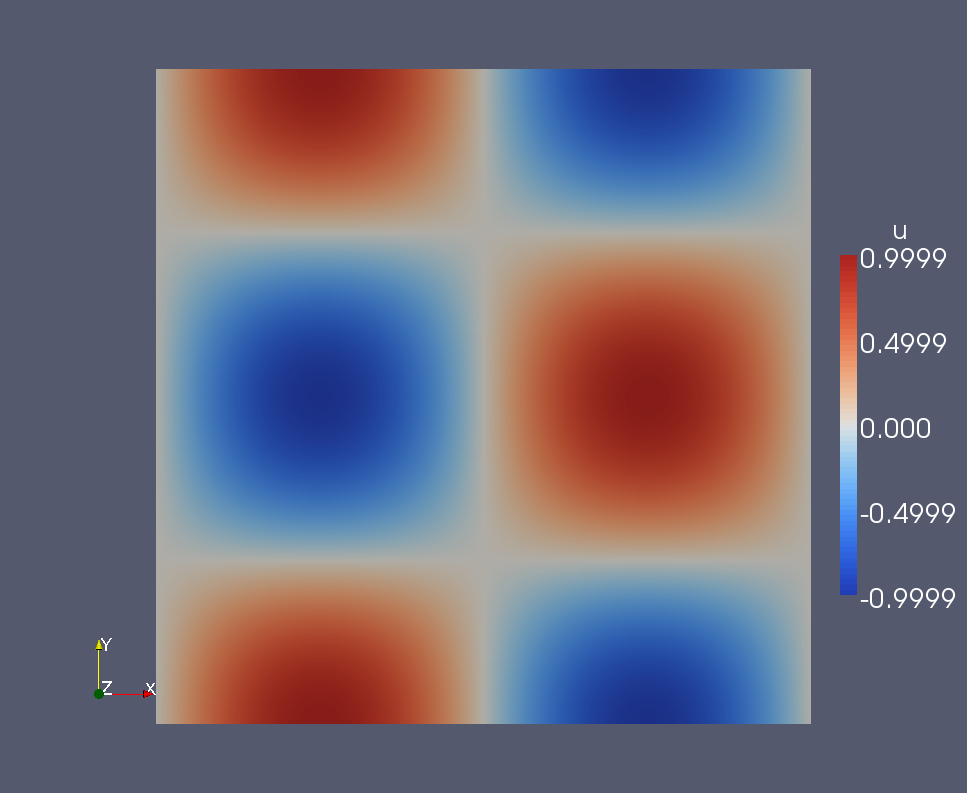
\includegraphics[width=.43\linewidth]{laplacian.png}}
  \subfigure[Elevation]{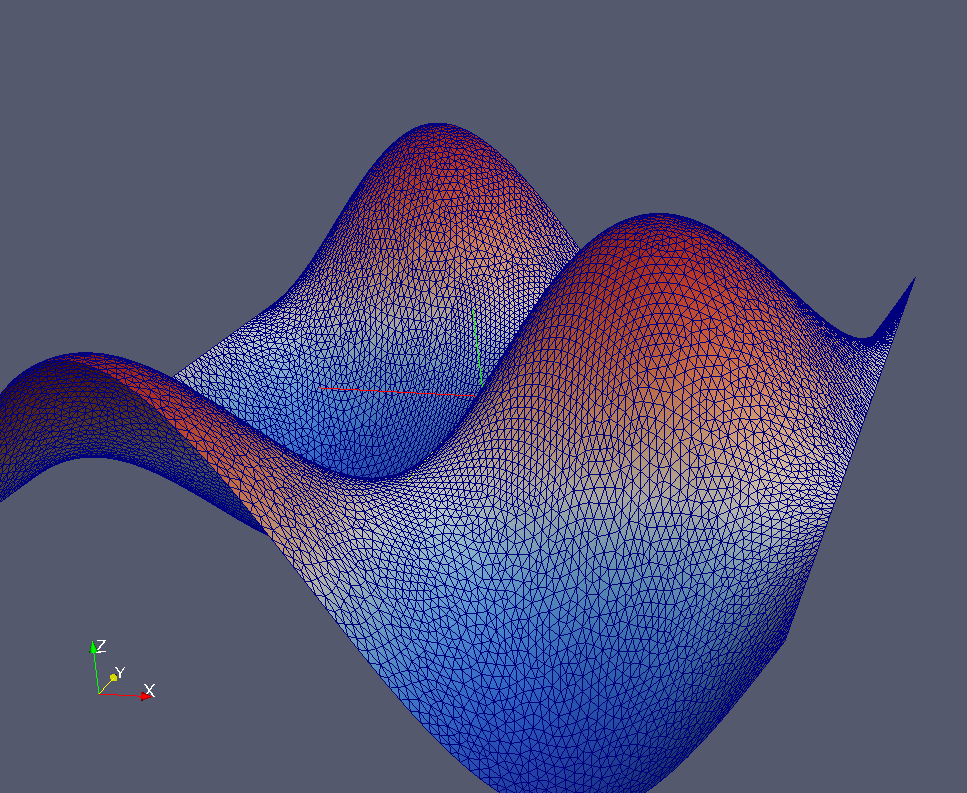
\includegraphics[width=.43\linewidth]{laplacian_warp.png}}
  \caption{Solution of problem~\ref{prob:3}}
  \label{fig:2}
\end{figure}

%%%%%%%%%%%%%%%%%%%%%%%%%%%%%%%%%%%%%%%%%%%%%%%%%%%%%%%%%%%%%%%%%%%%%%%%%%%%%%%%%%%%%%%%
Let's try a parallel computation using 3 processors. The following figures display the results using Paraview.
\begin{remark}
 You can modify the domain size in order to obtain a clearer figure by adding diffrent values to \lstinline!_xmin!    \lstinline!_ymin!   \lstinline!_xmax! and  \lstinline!_ymax!  in the definition of the mesh in \lstinline!laplacian.cpp!
 \end{remark}

 \begin{figure}[!h]%[htbp]
  \centering
  \subfigure[domain 1]{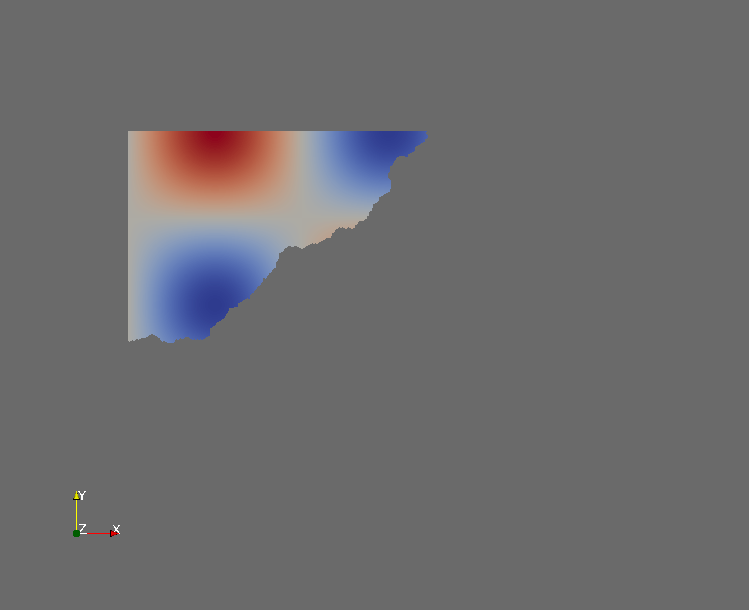
\includegraphics[width=.43\linewidth]{pngs/Laplacian/laplacian_1.png}}
  \subfigure[domain 2]{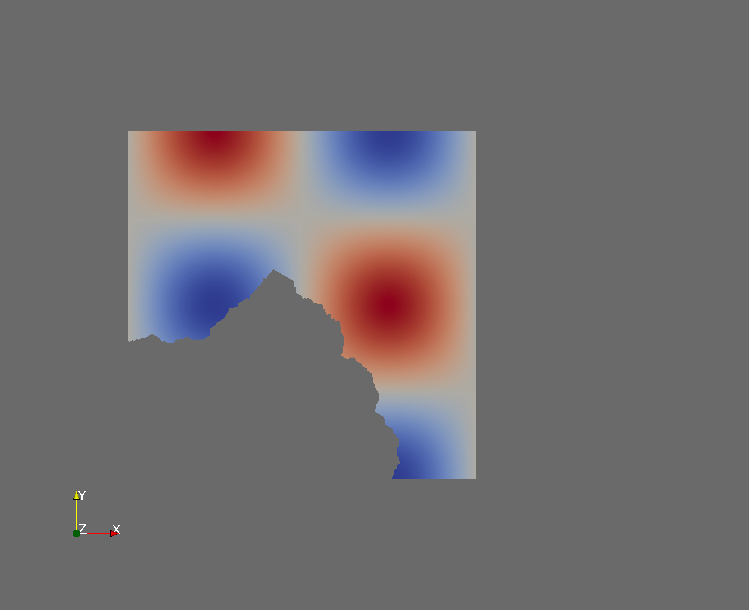
\includegraphics[width=.43\linewidth]{pngs/Laplacian/laplacian_2.png}}\\
  \subfigure[domain 3]{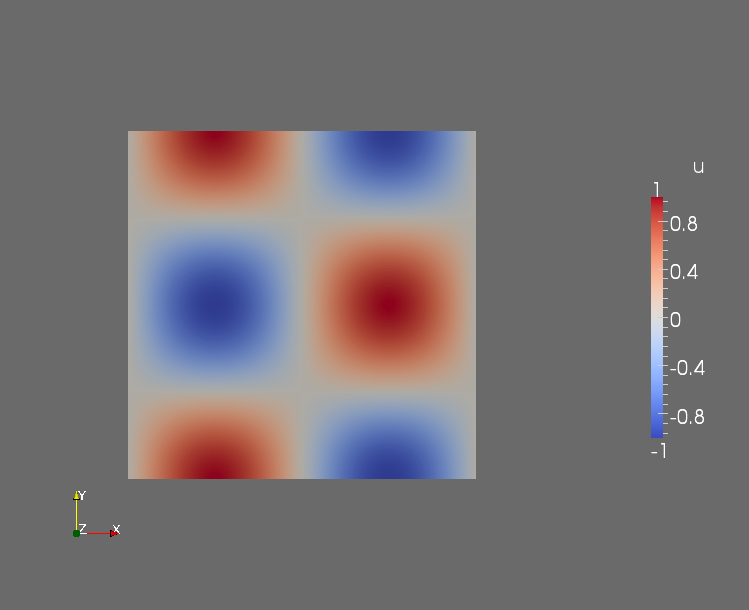
\includegraphics[width=.43\linewidth]{pngs/Laplacian/laplacian_3.png}}
  \subfigure[partition colored with pid]{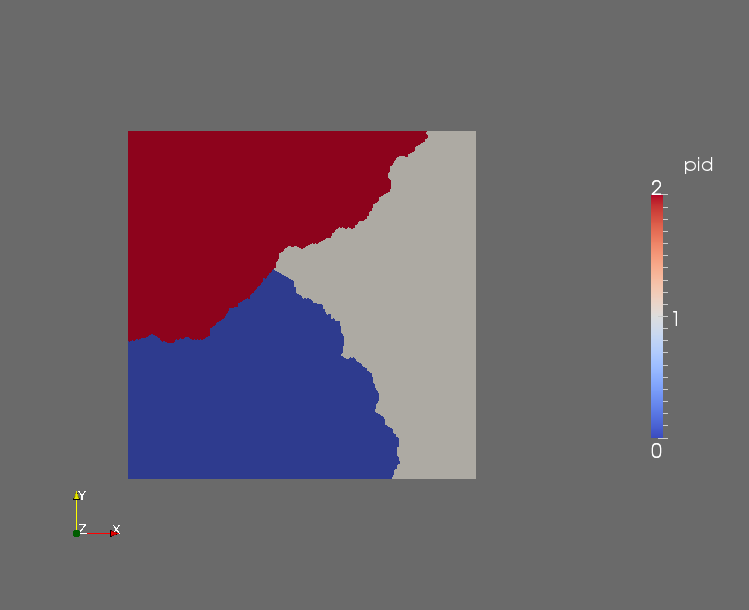
\includegraphics[width=.43\linewidth]{pngs/Laplacian/laplacian_Pid.png}}
  \caption{Solution of the laplacian problem}
  \label{fig:2}
\end{figure}
%%%%%%%%%%%%%%%%%%%%%%%%%%%%%%%%%%%%%%%%%%%%%%%%%%%%%%%%%%%%%%%%%%%%%%%%%%%%%%%%%%%%%%%%


\newpage

\subsection{Mixed formulation: the Stokes case}
\label{sec:mixed-form-stok}
\index{Stokes}
\subsubsection{Mathematical formulation}
\label{sec:math-form}

\index{Stokes!formulation!mathematical}
\marginpar{\lstinline!stokes.cpp!}  We are now interested in solving
the Stokes equations, we would like to solve for the following problem
in 2D
\begin{problem}
\label{prob:4}
 find $(\mathbf{u},p)$ such that
\begin{equation}
  \label{eq:22}
  - \mu \Delta \mathbf{u} +\nabla p = \mathbf{f}\quad \text{and}\quad \nabla \cdot \mathbf{u} = 0,\quad \text{in}\ \Omega = [-1;1]^2
\end{equation}
with
\begin{equation}
  \label{eq:24}
  \mathbf{f} = \mathbf{0}
\end{equation}
where $\mu$ being the viscosity. The following boundary conditions apply
\begin{equation}
  \label{eq:23}
  \mathbf{u}=\mathbf{1}_{|y=1}, \quad \mathbf{u}=\mathbf{0}_{|\partial \Omega \backslash \{(x,y) \in \Omega | y=1\}}
\end{equation}
\end{problem}

In problem (\ref{prob:2}), $p$ is known up to a constant $c$,
\emph{i.e.} if $p$ is a solution then $p+c$ is also solution. To
ensure uniqueness we impose the constraint that $p$ should have
zero-mean, \emph{i.e.}
\begin{equation}
  \label{eq:26}
  \int_\Omega p = 0
\end{equation}

The problem~\ref{prob:4} now reads
\begin{problem}
  \label{prob:5}
 find $(\mathbf{u},p,\lambda)$ such that
\begin{equation}
  \label{eq:34}
  - \mu \Delta \mathbf{u} +\nabla p = \mathbf{f}\quad, \quad \nabla \cdot \mathbf{u} + \lambda = 0, \quad \text{and}\quad \int_\Omega p = 0,\quad \text{in}\ \Omega = [-1;1]^2
\end{equation}
with
\begin{equation}
  \label{eq:35}
  \mathbf{f} = \mathbf{0}
\end{equation}
where $\mu$ being the viscosity. The following boundary conditions apply
\begin{equation}
  \label{eq:36}
  \mathbf{u}=\mathbf{1}_{|y=1}, \quad \mathbf{u}=\mathbf{0}_{|\partial \Omega \backslash \{(x,y) \in \Omega | y=1\}}
\end{equation}
\end{problem}

The functional framework is as follows, we look for $\mathbf{u}$ in
$H^1_0(\Omega)$ and $p$ in $L^2_0(\Omega)$. We shall not seek $p$ in
$L^2_0(\Omega)$ but rather in $L^2(\Omega)$ and use Lagrange
multipliers which live are the constants whose space we denote
$\mathbb{P}_0(\Omega)$, to enforce~(\ref{eq:26}).

Denote $\mathcal{X} = H^1_0(\Omega)\times
L^2(\Omega)\times\mathbb{P}_0(\Omega)$, the variational formulation
reads we look for $(\mathbf{u}, p, \lambda) \in \mathcal{X}$ for all
$(\mathbf{v},q,\nu) \in \mathcal{X}$
\begin{equation}
  \label{eq:25}
  \int_\Omega \mu \nabla \mathbf{u} : \nabla \mathbf{v} + \nabla \cdot \mathbf{v} p + \nabla \cdot \mathbf{u}\ q + q \lambda + p \nu  \ = \ \int_\Omega \mathbf{f} \cdot \mathbf{v}
\end{equation}

We build a triangulation $\Omega_h$ of $\Omega$, we choose compatible
(piecewise polynomial) discretisation spaces $X_h$ and $M_h$,
\emph{e.g.} the Taylor Hood element ($\mathbb{P}_N/\mathbb{P}_{N-1}$)
and we denote $\mathcal{X}_h=X_h\times M_h \times
\mathbb{P}_0(\Omega)$.  The discrete problem now reads, we look for
$(\mathbf{u}_h,p_h,\lambda_h) \in \mathcal{X}_h$ such that for all
$(\mathbf{v}_h,q_h,\nu_h) \in \mathcal{X}_h$
\begin{equation}
  \label{eq:27}
  \int_{\Omega_h} \mu \nabla \mathbf{u}_h \cdot \nabla \mathbf{v}_h + \nabla \cdot \mathbf{v}_h \ p_h + \nabla \cdot \mathbf{u}_h\ q_h + p_h \nu_h + q_h \lambda_h   = \ \int_{\Omega_h} \mathbf{f} \cdot \mathbf{v}_h
\end{equation}

The formulation~(\ref{eq:27}) leads to a linear system of the form
\begin{equation}
  \label{eq:28}
  \underbrace{\begin{pmatrix}
    A & B & 0\\
    B^T & 0 & C\\
    0 & C^T & 0
  \end{pmatrix}}_{\mathcal{A}}
\underbrace{
  \begin{pmatrix}
    \mathbf{u}_h\\
    p_h\\
    \lambda_h
  \end{pmatrix}}_{\mathcal{U}} =
\underbrace{\begin{pmatrix}
    F\\
    0\\
    0
  \end{pmatrix}}_{\mathcal{F}}
\end{equation}

where $A$ corresponds to the $(\mathbf{u},\mathbf{v})$ block, $B$ to
the $(\mathbf{u},q)$ block and $C$ to the $(p,\nu)$
block. $\mathcal{A}$ is a symetric positive definite matrix and thus
the system $\mathcal{A} \mathcal{U} = \mathcal{F}$ enjoys a unique
solution.

\subsubsection{Feel formulation}
\label{sec:feel-formulation}

\index{Stokes!formulation!feel}
Regarding the implementation of the Stokes problem~\ref{prob:4}, we
can start from the laplacian case, from
section~\ref{sec:defin-bilin-forms}. The implementation we choose to
display here defines and builds $\mathcal{X}_h$, $\mathcal{A}$,
$\mathcal{U}$ and $\mathcal{F}$.

We start by defining and building $\mathcal{X}_h$: first we define the
basis functions that will span each subspaces $X_h$, $M_h$ and
$\mathbb{P}_0(\Omega)$.

\lstinputlisting[linerange=marker1-endmarker1]{stokes/stokes.cpp}

note that on the \lstinline!typedef! we build a (MPL) vector of them. Now we are
ready to define the functionspace $\mathcal{X}_h$, much like in the
Laplacian case:

\lstinputlisting[linerange=marker2-endmarker2]{stokes/stokes.cpp}

Next we define a few types which are associated with $\mathcal{U}$,
$u$, $p$ and $\lambda$ respectively.

\lstinputlisting[linerange=marker3-endmarker3]{stokes/stokes.cpp}

Using these types we can instantiate elements of $\mathcal{X}_h$,
$X_h$, $M_h$ and $\mathbb{P}_0(\Omega_h)$ respectively:

\lstinputlisting[linerange=marker4-endmarker4]{stokes/stokes.cpp}

They will serve in the definition of the variational formulation. We
can now start assemble the various terms of the variational
formulation~(\ref{eq:27}). First we define some viscous stress tensor,
%$\tau(\mathbf{u}) = \frac{1}{2}(\nabla \mathbf{u} + \nabla \mathbf{u}^T)$,
$\tau(\mathbf{u}) = \nabla \mathbf{u}$,
associated with the trial and test functions
respectively

\lstinputlisting[linerange=marker5-endmarker5]{stokes/stokes.cpp}

Then we define the total stress tensor times the normal,
$\bar{\sigma}(\mathbf{u},p) \mathbf{n} = -p \mathbf{n} + 2 \mu \tau(\mathbf{u})
\mathbf{n}$ where $\mathbf{n}$ is the normal and $\bar{\sigma}(\mathbf{u},p) =
-p \mathbb{I} + 2 \mu \tau(\mathbf{u})$:

\lstinputlisting[linerange=marker6-endmarker6]{stokes/stokes.cpp}


We then form the matrix $\mathcal{A}$ starting with block $A$,  block $B$
block $C$ and finally the boundary conditions.


\lstinputlisting[linerange=marker7-endmarker7]{stokes/stokes.cpp}

The figure~\ref{fig:2} displays $p$ and $\mathbf{u}$ which are available in
\begin{unixcom}
  ls ~/feel/doc/tutorial/stokes/Simplex_2_1_2/P2/h_0.05
\end{unixcom}

\begin{figure}[htbp]
  \centering
  \subfigure[Colored with $p$, $h=0.05$]{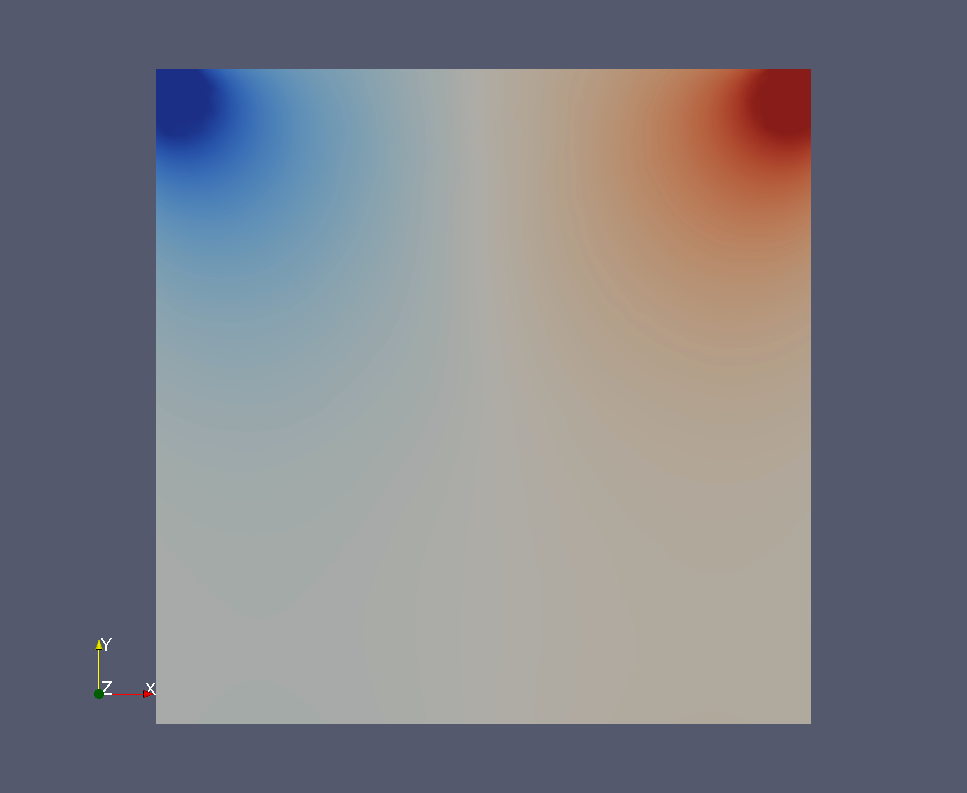
\includegraphics[width=.43\linewidth]{stokes-p.png}}
  \subfigure[Colored with $\|\mathbf{u}\|$ and the arrows associated to $\mathbf{u}$ colored with $p$]{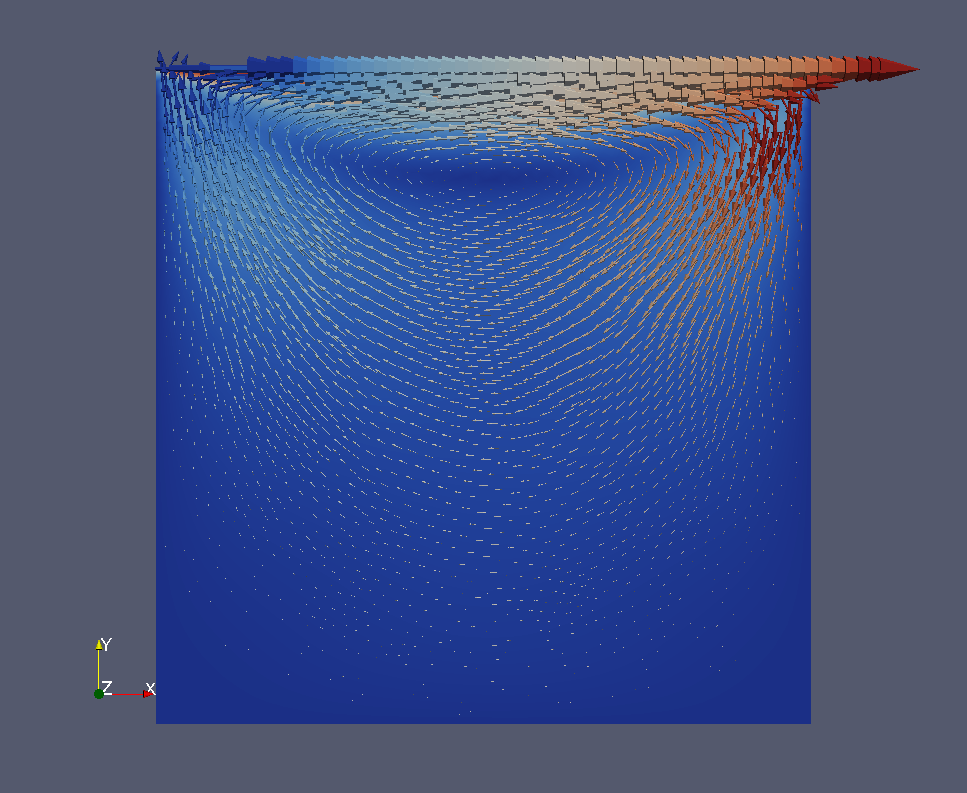
\includegraphics[width=.43\linewidth]{stokes-u.png}}
  \caption{Solution of problem~\ref{prob:4}}
  \label{fig:2}
\end{figure}

%%% Local Variables:
%%% coding: utf-8
%%% mode: latex
%%% TeX-PDF-mode: t
%%% TeX-parse-self: t
%%% x-symbol-8bits: nil
%%% TeX-auto-regexp-list: TeX-auto-full-regexp-list
%%% TeX-master: "../feel-manual"
%%% ispell-local-dictionary: "american"
%%% End:
